\chapter{La energía de las reacciones: combustión y energías de enlace}\label{ch:g11:reaction-energy}

Rompes el precinto de un calentador de manos y, un minuto después,
quema tanto que cuesta sostenerlo; aprietas una bolsa de frío
instantáneo y enfría un tobillo torcido; un autobús urbano funciona todo
el día con hidrógeno y solo deja vapor de agua tras de sí. Las
transformaciones químicas no solo convierten unas sustancias en otras:
liberan energía, o la absorben. ¿De dónde viene esa energía, y cuánta
puede dar un \omterm{def:g4:what-a-fire-needs:fuel}{combustible}?

\begin{recall}
En una \omterm{def:g8:combustion-and-fuels:complete}{combustión completa}, un \omterm{def:g4:what-a-fire-needs:fuel}{combustible} formado por carbono e
hidrógeno \omterm{def:g4:what-a-fire-needs:burning}{arde} en dioxígeno y da dióxido de carbono y agua
(\cref{ch:g8:combustion-and-fuels}). Un \omterm{def:g10:lewis-and-shape:covalent-bond}{enlace covalente} es un par de
\omterm{def:g9:inside-the-atom:nucleus}{electrones} compartido; las \omterm{def:g10:lewis-and-shape:lewis-structure}{estructuras de Lewis} muestran todos los
enlaces de una \omterm{def:g7:atoms-and-molecules:molecule}{molécula} (\cref{ch:g10:lewis-and-shape}). La \omterm{def:g10:the-mole:amount}{cantidad de
sustancia} se cuenta en \omterm{def:g10:the-mole:amount}{moles} (\cref{ch:g10:the-mole}).
\end{recall}

\begin{omfigure}
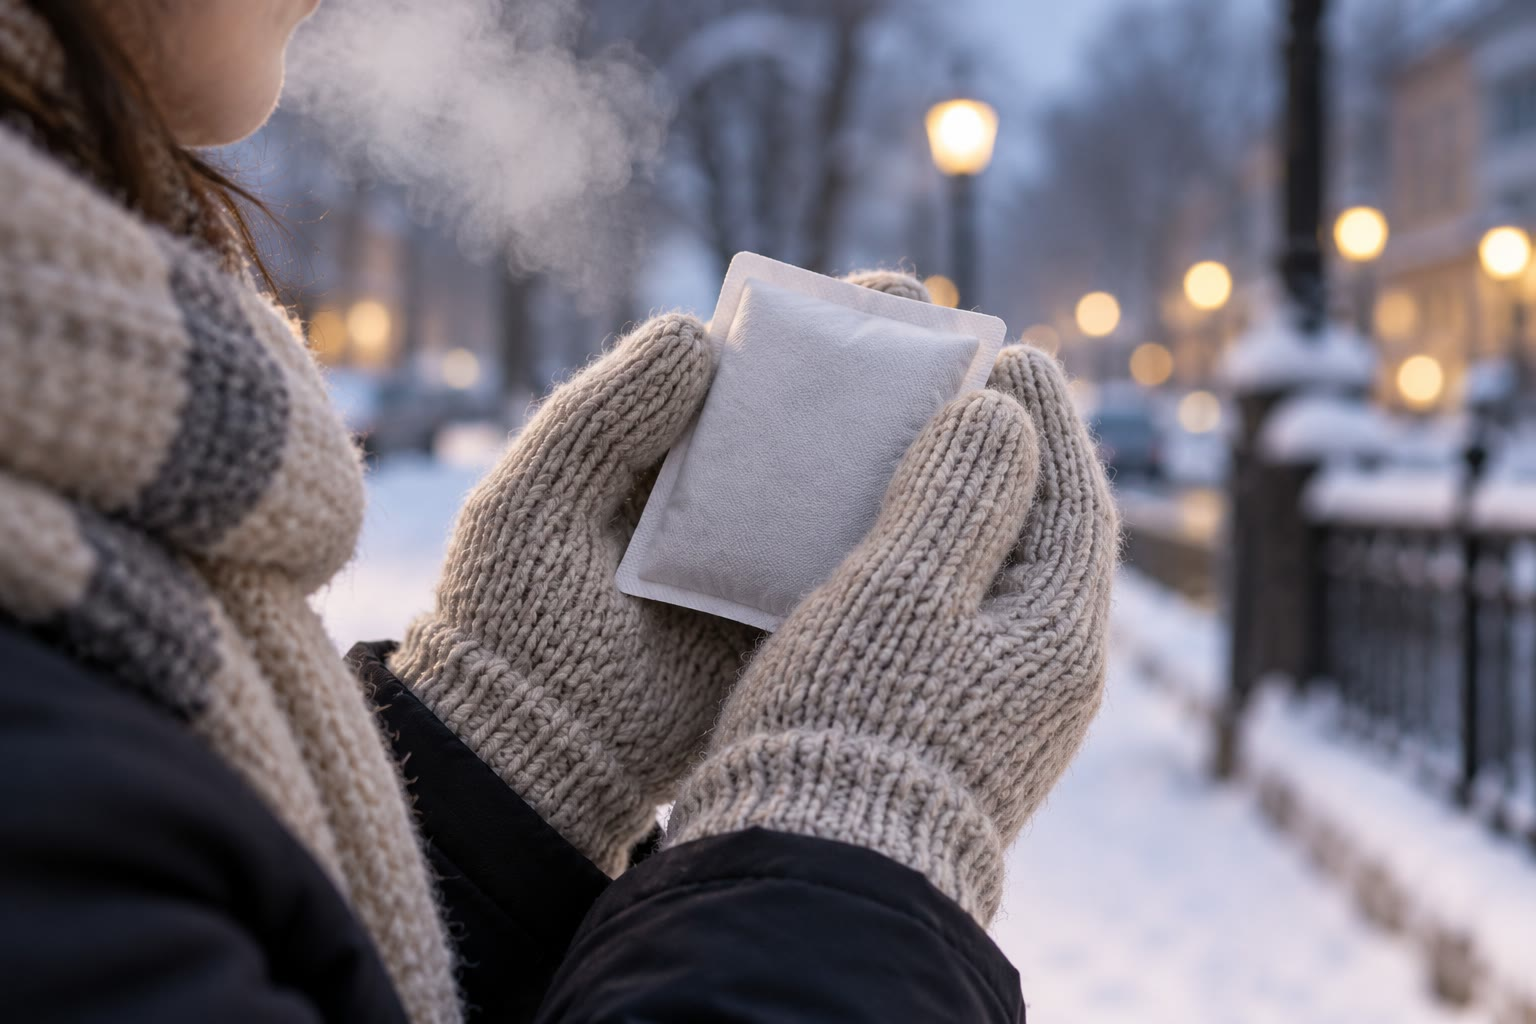
\includegraphics[width=0.45\linewidth]{images/book1/ai/g11-hand-warmers.jpg}

{\small Un calentador de manos: una reacción dentro de la bolsita libera
calor.}
\end{omfigure}

\section{Transformaciones exotérmicas y endotérmicas}

\begin{definition}[Exotérmica, endotérmica]\label{def:g11:reaction-energy:exothermic}
Una transformación es \emph{exotérmica}\index{exotermica@exotérmica} si libera
energía a su entorno, por lo general en forma de calor: el entorno se
calienta. Es \emph{endotérmica}\index{endotermica@endotérmica} si absorbe energía de
su entorno: este se enfría, o la transformación necesita que se la
caliente para continuar.
\end{definition}

\begin{example}[Calor y frío]\label{ex:g11:reaction-energy:packs}
Las combustiones son \omterm{def:g11:reaction-energy:exothermic}{exotérmicas}, y también lo es la reacción lenta del
hierro en polvo con el dioxígeno del \omterm{def:g4:air-a-mixture-of-gases:air}{aire} dentro de un calentador de
manos. La disolución del nitrato de amonio en agua, que se usa en las
bolsas de frío, es \omterm{def:g11:reaction-energy:exothermic}{endotérmica}; también lo es la descomposición de la
caliza en cal viva y dióxido de carbono, que solo se produce en un horno
muy caliente.
\end{example}

\begin{omfigure}
\begin{tikzpicture}[font=\small]
  \begin{scope}
    \draw[->] (0,0) -- (0,3.2) node[above] {energía};
    \draw[very thick, omDef] (0.5,2.5) -- (2.3,2.5) node[right, text=black] {reactivos};
    \draw[very thick, omProp] (0.5,0.8) -- (2.3,0.8) node[right, text=black] {productos};
    \draw[->, thick, omThm] (1.4,2.45) -- (1.4,0.85);
    \node[omThm, anchor=west, align=left] at (1.5,1.65) {energía\\ liberada};
    \node[anchor=north] at (1.6,-0.15) {\textbf{exotérmica}};
  \end{scope}
  \begin{scope}[xshift=6cm]
    \draw[->] (0,0) -- (0,3.2) node[above] {energía};
    \draw[very thick, omDef] (0.5,0.8) -- (2.3,0.8) node[right, text=black] {reactivos};
    \draw[very thick, omProp] (0.5,2.5) -- (2.3,2.5) node[right, text=black] {productos};
    \draw[->, thick, omDef] (1.4,0.85) -- (1.4,2.45);
    \node[omDef, anchor=west, align=left] at (1.5,1.65) {energía\\ absorbida};
    \node[anchor=north] at (1.6,-0.15) {\textbf{endotérmica}};
  \end{scope}
\end{tikzpicture}

{\small Diagramas de energía. En una reacción \omterm{def:g11:reaction-energy:exothermic}{exotérmica}, los productos
tienen menos energía que los \omterm{def:g7:chemical-reactions:reactant}{reactivos}, y la diferencia se libera; en
una \omterm{def:g11:reaction-energy:exothermic}{endotérmica} tienen más, y hay que aportarla.}
\end{omfigure}

\section{La energía liberada por una combustión}

\begin{definition}[Energía molar de combustión]\label{def:g11:reaction-energy:combustion-energy}
La \emph{energía molar de combustión}\index{energia molar de combustion@energía molar de combustión}
$E_c$ de un \omterm{def:g4:what-a-fire-needs:fuel}{combustible} es la energía que libera la \omterm{def:g8:combustion-and-fuels:complete}{combustión completa}
de un \omterm{def:g10:the-mole:amount}{mol} de él, en \si{kJ/mol}, con el agua formada en estado líquido.
\end{definition}

\begin{proposition}[Energía liberada por $n$ moles]\label{prop:g11:reaction-energy:n-moles}
% ledger: dch:CH4
La \omterm{def:g8:combustion-and-fuels:complete}{combustión completa} de una cantidad $n$ de \omterm{def:g4:what-a-fire-needs:fuel}{combustible} libera la
energía $Q = n \times E_c$. Para el metano, $E_c = \qty{890.7}{kJ/mol}$:
al quemar \qty{1.00}{mol} (\qty{16.0}{g}) se liberan unos
\qty{891}{kJ}.
\end{proposition}

\begin{proof}
Cada \omterm{def:g10:the-mole:amount}{mol} de \omterm{def:g4:what-a-fire-needs:fuel}{combustible} quemado libera $E_c$; $n$ \omterm{def:g10:the-mole:amount}{moles} liberan $n$
veces más.
\end{proof}

\begin{inthelab}[Calentar agua con una lamparilla de alcohol]
% ledger: cp:water
Se pesa una lamparilla de etanol y se enciende debajo de una lata
metálica que contiene \qty{200}{g} de agua, con un termómetro dentro.
Cuando el agua se ha calentado \qty{25}{\celsius}, se apaga la llama y
se vuelve a pesar la lamparilla: ha perdido \qty{1.50}{g} de etanol. La
energía que ha recibido el agua se calcula con la fórmula de física
$Q = m\, c\, \Delta\theta$, donde $c = \qty{4.18}{J/(g.\celsius)}$ es el
calor específico del agua. Queda muy por debajo de la energía que podría
liberar el etanol: gran parte del calor calienta el \omterm{def:g4:air-a-mixture-of-gases:air}{aire}, la lata y la
lamparilla, y una parte del etanol \omterm{def:g4:what-a-fire-needs:burning}{arde} de forma incompleta.
\end{inthelab}

\begin{omfigure}
\begin{tikzpicture}[font=\small]
  % spirit burner
  \fill[black!8, draw=black!60] (-0.6,0) rectangle (0.6,0.7);
  \fill[cyan!15] (-0.55,0.05) rectangle (0.55,0.45);
  \fill[black!40] (-0.06,0.7) rectangle (0.06,0.95);
  \fill[orange!70!yellow] (0,0.95) .. controls (-0.25,1.25) and (-0.1,1.6) .. (0,1.85)
    .. controls (0.1,1.6) and (0.25,1.25) .. (0,0.95);
  \fill[yellow!40] (0,1.0) .. controls (-0.1,1.2) and (-0.05,1.4) .. (0,1.5)
    .. controls (0.05,1.4) and (0.1,1.2) .. (0,1.0);
  % tripod and can
  \draw[black!60, line width=1pt] (-1.1,0) -- (-0.9,2.1) (1.1,0) -- (0.9,2.1);
  \draw[black!60, line width=1.2pt] (-1.1,2.1) -- (1.1,2.1);
  \fill[black!15, draw=black!60] (-0.8,2.1) rectangle (0.8,3.7);
  \fill[omWater] (-0.75,2.15) rectangle (0.75,3.3);
  % thermometer
  \pic at (0.35,2.35) {thermometer};
  \draw[omProp, thick, <-] (0.6,0.35) -- (2.0,0.35) node[right, text=black]
    {lamparilla de alcohol (etanol)};
  \draw[omProp, thick, <-] (0.8,2.9) -- (2.0,2.9) node[right, text=black]
    {lata: \qty{200}{g} de agua};
  \draw[omProp, thick, <-] (0.45,5.0) -- (2.0,5.0) node[right, text=black]
    {termómetro};
\end{tikzpicture}

{\small Medir la energía que da un \omterm{def:g4:what-a-fire-needs:fuel}{combustible}: una lamparilla de \omterm{def:g11:functional-groups:alcohol}{alcohol}
calienta una lata de agua cuyo aumento de temperatura se mide.}
\end{omfigure}


\begin{example}[La lamparilla en cifras]\label{ex:g11:reaction-energy:burner}
% ledger: cp:water, dch:C2H5OH, aw:C, aw:H, aw:O
El agua recibió $Q = 200 \times 4.18 \times 25 = \qty{2.09e4}{J}$, es
decir, \qty{20.9}{kJ}. El etanol quemado, \qty{1.50}{g}, son
$1.50 / 46.0 = \qty{0.0326}{mol}$; con $E_c = \qty{1367.6}{kJ/mol}$
podría liberar $0.0326 \times 1367.6 = \qty{44.6}{kJ}$. Solo
$20.9 / 44.6 \approx \qty{47}{\percent}$ llegó al agua.
\end{example}

\section{Las energías de enlace}

\begin{definition}[Energía de enlace]\label{def:g11:reaction-energy:bond-energy}
La \emph{energía de enlace}\index{energia de enlace@energía de enlace} de un \omterm{def:g10:lewis-and-shape:covalent-bond}{enlace
covalente} es la energía necesaria para romper un \omterm{def:g10:the-mole:amount}{mol} de esos enlaces,
estando las \omterm{def:g7:atoms-and-molecules:molecule}{moléculas} y los \omterm{def:g7:atoms-and-molecules:atom}{átomos} en estado gaseoso. Las tablas dan
valores medios, medidos en muchas \omterm{def:g7:atoms-and-molecules:molecule}{moléculas}, en \si{kJ/mol}.
\end{definition}

\begin{omfigure}
\small
% ledger: be:H-H, be:C-H, be:N-H, be:O-H, be:H-Cl, be:C-C, be:CC-double, be:C-O, be:CO-double, be:NN-triple, be:OO-double, be:Cl-Cl
\begin{tabular}{lr@{\qquad}lr@{\qquad}lr}
\hline
enlace & \si{kJ/mol} & enlace & \si{kJ/mol} & enlace & \si{kJ/mol} \\
\hline
\ce{H-H} & 436 & \ce{C-C} & 345 & \ce{O=O} & 498 \\
\ce{C-H} & 415 & \ce{C=C} & 611 & \ce{N#N} & 946 \\
\ce{N-H} & 390 & \ce{C-O} & 350 & \ce{Cl-Cl} & 243 \\
\ce{O-H} & 464 & \ce{C=O} & 741 & \ce{H-Cl} & 432 \\
\hline
\end{tabular}\par\medskip

{\small \omterm{def:g11:reaction-energy:bond-energy}{Energías de enlace} medias. Romper un enlace siempre cuesta
energía; formarlo devuelve la misma energía.}
\end{omfigure}

\begin{omfigure}
\begin{tikzpicture}[font=\small, x=1cm, y=0.0015cm]
  \draw[->] (0,-850) -- (0,2900) node[above] {energía (\si{kJ})};
  \draw[very thick, black!60] (0.4,2656) -- (3.9,2656);
  \node[anchor=west] at (4.0,2656) {átomos separados: \ce{C + 4H + 4O}};
  \draw[very thick, omDef] (0.4,0) -- (3.9,0);
  \node[anchor=west] at (4.0,0) {\ce{CH4 + 2O2}};
  \draw[very thick, omProp] (0.4,-682) -- (3.9,-682);
  \node[anchor=west] at (4.0,-682) {\ce{CO2 + 2H2O}};
  \draw[->, thick, omDef] (1.0,30) -- (1.0,2626);
  \node[omDef, anchor=west, align=left] at (1.05,1500) {romper 4 \ce{C-H}\\ y 2 \ce{O=O}:\\ $+\qty{2656}{kJ}$};
  \draw[->, thick, omProp] (3.4,2626) -- (3.4,-652);
  \node[omProp, anchor=west, align=left] at (3.45,1200) {formar 2 \ce{C=O}\\ y 4 \ce{O-H}:\\ $-\qty{3338}{kJ}$};
  \draw[<->, omThm, thick] (0.6,-10) -- (0.6,-672);
  \node[omThm, anchor=west] at (0.65,-341) {$E_r \approx \qty{-682}{kJ}$};
\end{tikzpicture}

{\small La \omterm{def:g4:what-a-fire-needs:burning}{combustión} del metano en dos etapas imaginarias, con \omterm{def:g11:reaction-energy:bond-energy}{energías
de enlace} medias: romper todos los enlaces y formar después los nuevos.
La estimación, \qty{-682}{kJ} por \omterm{def:g10:the-mole:amount}{mol} de metano, es \omterm{def:g11:reaction-energy:exothermic}{exotérmica}.}
\end{omfigure}

\begin{proposition}[Estimar una energía de reacción]\label{prop:g11:reaction-energy:estimate}
Para una reacción entre gases, la energía absorbida, $E_r$ (negativa si
se libera energía), es aproximadamente
\[
  E_r \approx \sum E(\text{enlaces rotos}) - \sum E(\text{enlaces formados}) .
\]
Si $E_r < 0$, al formar los enlaces nuevos se libera más energía de la
necesaria para romper los antiguos: la reacción es \omterm{def:g11:reaction-energy:exothermic}{exotérmica}.
\end{proposition}

\begin{proof}
Se imagina la reacción en dos etapas: se rompen todos los enlaces de los
\omterm{def:g7:chemical-reactions:reactant}{reactivos}, lo que cuesta la primera suma y deja \omterm{def:g7:atoms-and-molecules:atom}{átomos} separados; después
se forman los enlaces de los productos, lo que devuelve la segunda suma.
El resultado es solo una estimación, porque las tablas dan medias sobre
muchas \omterm{def:g7:atoms-and-molecules:molecule}{moléculas}.
\end{proof}

\begin{method}[Estimar una energía de reacción con las energías de enlace]\label{met:g11:reaction-energy:bonds}
\begin{enumerate}
  \item Escribir la \omterm{def:g8:balanced-equations:equation}{ecuación ajustada} y la \omterm{def:g10:lewis-and-shape:lewis-structure}{estructura de Lewis} de cada
        \omterm{def:g7:atoms-and-molecules:molecule}{molécula}.
  \item Contar los enlaces de cada clase rotos en los \omterm{def:g7:chemical-reactions:reactant}{reactivos} y
        formados en los productos, con los coeficientes.
  \item Sumar las energías de los enlaces rotos y restar las de los
        enlaces formados.
  \item Concluir: un resultado negativo indica una reacción \omterm{def:g11:reaction-energy:exothermic}{exotérmica}.
\end{enumerate}
\end{method}

\begin{example}[El hidrógeno y el cloro]\label{ex:g11:reaction-energy:hcl}
% ledger: be:H-H, be:Cl-Cl, be:H-Cl
Para \ce{H2 + Cl2 -> 2HCl}: se rompen un \ce{H-H} y un \ce{Cl-Cl},
$436 + 243 = \qty{679}{kJ}$; se forman dos \ce{H-Cl}, $2 \times 432 =
\qty{864}{kJ}$. Así, $E_r \approx 679 - 864 = \qty{-185}{kJ}$ por \omterm{def:g10:the-mole:amount}{mol} de
reacción: \omterm{def:g11:reaction-energy:exothermic}{exotérmica}.
\end{example}


\begin{remark}[Estimación y medida]\label{rem:g11:reaction-energy:compare}
% ledger: dch:CH4
La energía medida que libera la \omterm{def:g4:what-a-fire-needs:burning}{combustión} de un \omterm{def:g10:the-mole:amount}{mol} de metano es de
\qty{890.7}{kJ}, mayor que la estimación. Tres razones: los enlaces
\ce{C=O} del dióxido de carbono son más fuertes que el \ce{C=O} medio
de la tabla; el valor medido corresponde al agua líquida, y al
condensarse el vapor de agua se libera más energía; y las \omterm{def:g11:reaction-energy:bond-energy}{energías de
enlace} medias solo son medias. El método de las \omterm{def:g11:reaction-energy:bond-energy}{energías de enlace} da
el signo y el orden de magnitud, no el valor exacto.
\end{remark}

\section{Comparar combustibles}

\begin{omfigure}
\begin{tikzpicture}
\begin{axis}[xbar, width=0.78\linewidth, height=5.4cm, xmin=0, xmax=160,
    xlabel={energía liberada por kilogramo quemado (\si{MJ/kg})},
    symbolic y coords={ethanol, octane, propane, methane, hydrogen},
    yticklabels={etanol, octano, propano, metano, hidrógeno},
    ytick=data, bar width=10pt, nodes near coords,
    nodes near coords style={font=\footnotesize, /pgf/number format/fixed,
      /pgf/number format/precision=1, /pgf/number format/fixed zerofill},
    tick label style={font=\small}, label style={font=\small},
    axis lines*=left, xmajorgrids, grid style={gray!20}, enlarge y limits=0.15]
  % ledger: dch:C2H5OH, dfh:C8H18, dfh:CO2, dfh:H2O-l, dch:C3H8, dch:CH4 (per kg with the book's molar masses)
  \addplot[fill=omProp!55, draw=omProp] coordinates {(29.7,ethanol) (48.0,octane)
    (50.4,propane) (55.7,methane) (142.9,hydrogen)};
\end{axis}
\end{tikzpicture}

{\small Energía liberada por la \omterm{def:g8:combustion-and-fuels:complete}{combustión completa} de un kilogramo de
cinco \omterm{def:g4:what-a-fire-needs:fuel}{combustibles} (agua formada líquida). El hidrógeno es, con mucho,
el que más da por kilogramo; el etanol, ya en parte ``quemado'' (contiene
oxígeno), el que menos.}
\end{omfigure}

\begin{example}[Dióxido de carbono por megajulio]\label{ex:g11:reaction-energy:co2}
% ledger: dch:CH4, dch:C2H5OH
La \omterm{def:g4:what-a-fire-needs:burning}{combustión} de un \omterm{def:g10:the-mole:amount}{mol} de metano libera \qty{890.7}{kJ} y un \omterm{def:g10:the-mole:amount}{mol} de
dióxido de carbono, \qty{44.0}{g}. Por cada megajulio, \qty{1000}{kJ},
libera $44.0 \times 1000 / 890.7 = \qty{49.4}{g}$ de dióxido de carbono.
El etanol, con dos \omterm{def:g10:the-mole:amount}{moles} de dióxido de carbono por cada
\qty{1367.6}{kJ}, libera $88.0 \times 1000 / 1367.6 = \qty{64.3}{g}$ por
megajulio. El hidrógeno no libera nada: su único producto es el agua.
\end{example}

\begin{omfigure}
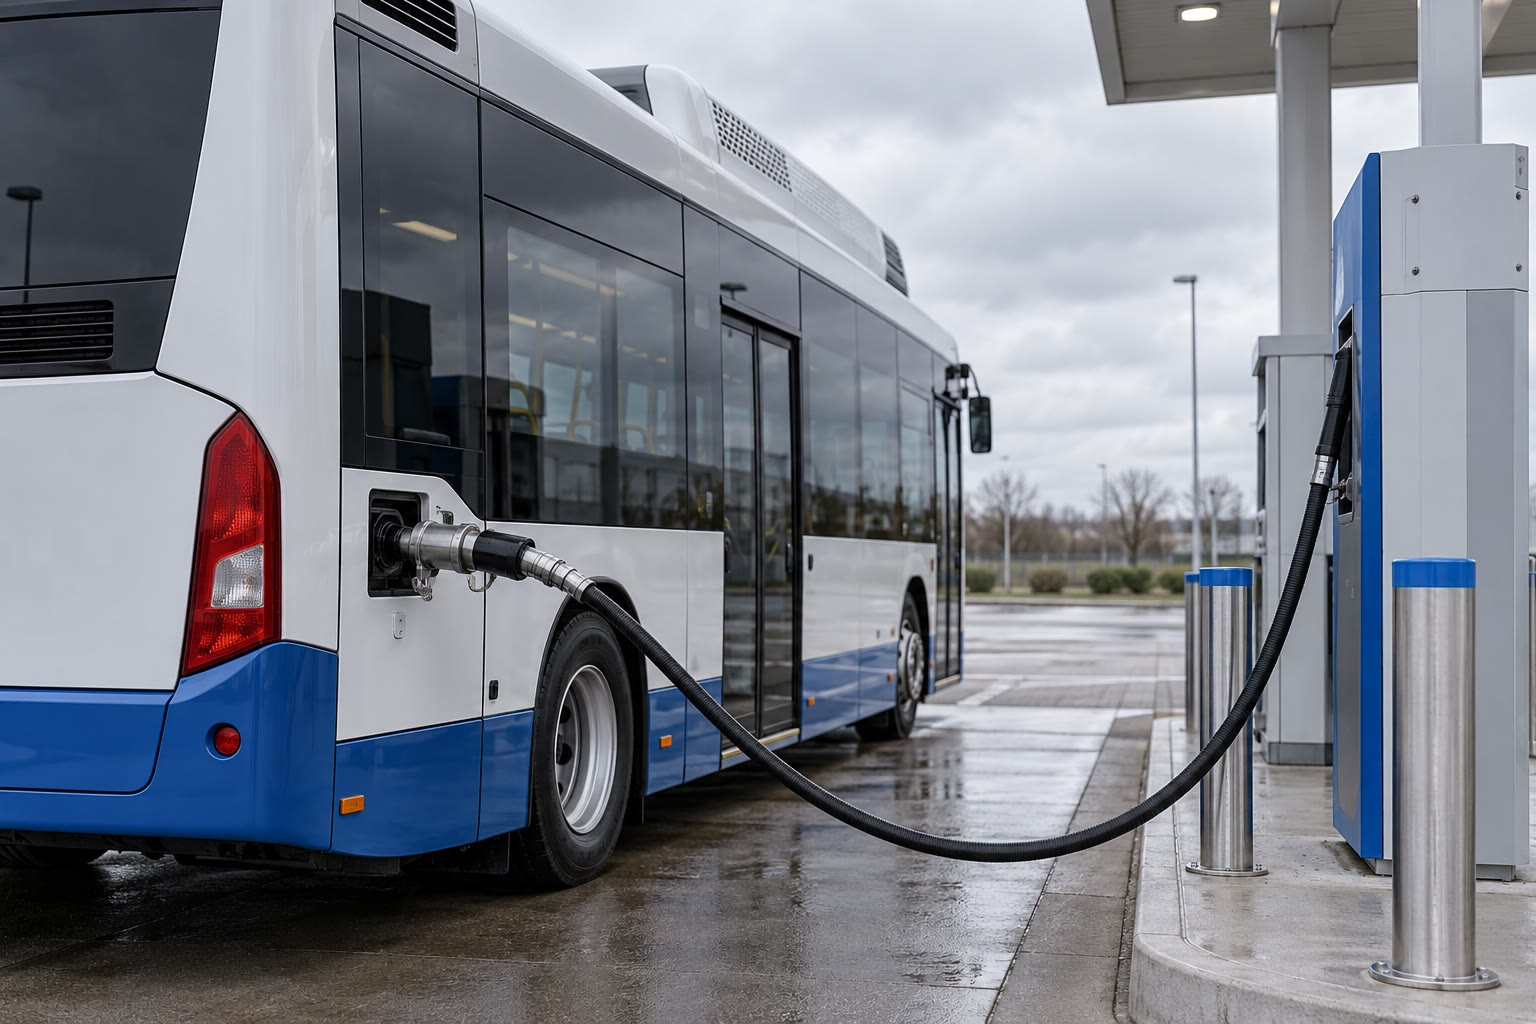
\includegraphics[width=0.5\linewidth]{images/book1/ai/g11-hydrogen-bus.jpg}

{\small Un autobús en una estación de hidrógeno: su \omterm{def:g4:what-a-fire-needs:fuel}{combustible} solo
libera agua.}
\end{omfigure}

\begin{safety}{\ghs[0.82cm]{GHS02}\ghs[0.82cm]{GHS07}}
% ledger: ghs:ethanol
El etanol es muy inflamable e irrita los ojos. Una lamparilla de \omterm{def:g11:functional-groups:alcohol}{alcohol}
se llena lejos de cualquier llama, nunca se rellena mientras está
caliente, y la usa el profesor sobre una placa resistente al calor.
\end{safety}

\section{Ejercicios}


\begin{exercise}[$\star$]\label{exo:g11:reaction-energy:1}
¿\omterm{def:g11:reaction-energy:exothermic}{Exotérmica} o \omterm{def:g11:reaction-energy:exothermic}{endotérmica}: la madera que \omterm{def:g4:what-a-fire-needs:burning}{arde}; el hielo que se funde;
una bolsa de frío que se aprieta; un calentador de manos que se calienta;
una hoja verde que fabrica azúcar con la luz del Sol?
\end{exercise}

\begin{exercise}[$\star$]\label{exo:g11:reaction-energy:2}
% ledger: dch:CH4
¿Qué energía libera la \omterm{def:g8:combustion-and-fuels:complete}{combustión completa} de \qty{3.0}{mol} de metano?
\end{exercise}

\begin{exercise}[$\star$]\label{exo:g11:reaction-energy:3}
En el diagrama de energía de una reacción \omterm{def:g11:reaction-energy:exothermic}{exotérmica}, ¿qué tiene más
energía, los \omterm{def:g7:chemical-reactions:reactant}{reactivos} o los productos? ¿Adónde va la diferencia?
\end{exercise}

\begin{exercise}[$\star$]\label{exo:g11:reaction-energy:4}
% ledger: dch:C2H5OH
¿Qué energía libera la \omterm{def:g8:combustion-and-fuels:complete}{combustión completa} de \qty{100}{g} de etanol?
\end{exercise}

\begin{exercise}[$\star$]\label{exo:g11:reaction-energy:5}
¿Qué es una \omterm{def:g11:reaction-energy:bond-energy}{energía de enlace}? ¿Por qué romper un enlace siempre cuesta
energía?
\end{exercise}

\begin{exercise}[$\star\star$]\label{exo:g11:reaction-energy:6}
Estima, con las \omterm{def:g11:reaction-energy:bond-energy}{energías de enlace}, la energía de la reacción
\ce{2H2 + O2 -> 2H2O}, todo en estado gaseoso. ¿Es \omterm{def:g11:reaction-energy:exothermic}{exotérmica}?
\end{exercise}

\begin{exercise}[$\star\star$]\label{exo:g11:reaction-energy:7}
Estima la energía de la \omterm{def:g4:what-a-fire-needs:burning}{combustión} del etanol, \ce{C2H5OH + 3O2 ->
2CO2 + 3H2O}, con las \omterm{def:g11:reaction-energy:bond-energy}{energías de enlace} (dibuja primero la \omterm{def:g10:lewis-and-shape:lewis-structure}{estructura
de Lewis} del etanol), y compárala con el valor medido de
\qty{1367.6}{kJ/mol}.
\end{exercise}

\begin{exercise}[$\star\star$]\label{exo:g11:reaction-energy:8}
% ledger: dch:C3H8, dch:CH4
Calcula la energía liberada por kilogramo de propano
(\qty{2219.2}{kJ/mol}) y de metano. Compáralas con el diagrama de
barras.
\end{exercise}

\begin{exercise}[$\star\star$]\label{exo:g11:reaction-energy:9}
% ledger: cp:water, dch:CH4
Una cocina de gas calienta \qty{1.50}{L} de agua (\qty{1500}{g}) de
\qty{15}{\celsius} a \qty{100}{\celsius}. ¿Qué energía recibe el agua?
¿Qué masa de metano se quema si toda la energía llega al agua? ¿Y si
solo llega la mitad?
\end{exercise}

\begin{exercise}[$\star\star$]\label{exo:g11:reaction-energy:10}
Con el diagrama de barras, ordena los \omterm{def:g4:what-a-fire-needs:fuel}{combustibles} por energía por
kilogramo. ¿Qué masa de hidrógeno da la misma energía que \qty{1.0}{kg}
de octano?
\end{exercise}

\begin{exercise}[$\star\star$]\label{exo:g11:reaction-energy:11}
Estima la energía de \ce{N2 + 3H2 -> 2NH3}, todo en estado gaseoso.
¿\omterm{def:g11:reaction-energy:exothermic}{Exotérmica} o \omterm{def:g11:reaction-energy:exothermic}{endotérmica}?
\end{exercise}

\begin{exercise}[$\star\star\star$]\label{exo:g11:reaction-energy:12}
% ledger: cp:water, dch:C2H5OH
En un experimento con una lamparilla de \omterm{def:g11:functional-groups:alcohol}{alcohol}, \qty{250}{g} de agua se
calientan \qty{20}{\celsius} mientras \omterm{def:g4:what-a-fire-needs:burning}{arden} \qty{1.20}{g} de etanol.
Calcula la energía recibida por el agua, la energía que podría liberar
el etanol y el \omterm{def:g10:synthesis-yield:yield}{rendimiento} del calentamiento. Nombra tres causas de las
pérdidas.
\end{exercise}

\begin{exercise}[$\star\star\star$]\label{exo:g11:reaction-energy:13}
% ledger: dfh:C8H18, dfh:CO2, dfh:H2O-l, dch:C3H8
El octano libera \qty{5470}{kJ/mol}, y el propano, \qty{2219.2}{kJ/mol}.
Escribe sus ecuaciones de \omterm{def:g4:what-a-fire-needs:burning}{combustión} y calcula la masa de dióxido de
carbono que libera cada uno por megajulio. Compárala con la del metano,
\qty{49.4}{g}.
\end{exercise}

\begin{exercise}[$\star\star\star$]\label{exo:g11:reaction-energy:14}
Tanto para el metano como para el etanol, la estimación con las \omterm{def:g11:reaction-energy:bond-energy}{energías
de enlace} es menor que la energía liberada medida. Da las razones, y
explica por qué la estimación sigue siendo útil.
\end{exercise}

\begin{exercise}[$\star\star\star$]\label{exo:g11:reaction-energy:15}
Estima la energía de \ce{2H2O -> 2H2 + O2}, todo en estado gaseoso. ¿Por
qué hay que aportar energía (por ejemplo, en forma de electricidad) para
fabricar hidrógeno a partir del agua? Explica por qué se dice que el
hidrógeno es una manera de \emph{almacenar} energía, más que una fuente
de energía.
\end{exercise}

\section{Problema: ¿Qué combustible para el autobús urbano?}

\begin{problem}[{Problema de fin de semana --- metano, etanol, octano o
hidrógeno: ¿cuál da más energía por kilogramo, y cuánto dióxido de
carbono por megajulio?}]
\label{pb:g11:reaction-energy:1}
% ledger: dch:CH4, dch:C2H5OH, dfh:C8H18, dfh:CO2, dfh:H2O-l, be:C-H, be:OO-double, be:CO-double, be:O-H
Una ciudad compara cuatro \omterm{def:g4:what-a-fire-needs:fuel}{combustibles} para sus autobuses: el metano
(gas natural), el etanol, el octano (de la gasolina) y el hidrógeno. Las
energías liberadas por la \omterm{def:g8:combustion-and-fuels:complete}{combustión completa} de un \omterm{def:g10:the-mole:amount}{mol} son: metano
\qty{890.7}{kJ}, etanol \qty{1367.6}{kJ}, octano \qty{5470}{kJ},
hidrógeno \qty{285.8}{kJ}, con el agua formada en estado líquido.

\medskip
\noindent\textbf{Parte I --- Ecuaciones de \omterm{def:g4:what-a-fire-needs:burning}{combustión}.}
\begin{enumerate}
  \item Escribe la ecuación de la \omterm{def:g8:combustion-and-fuels:complete}{combustión completa} del metano.
  \item La del etanol, \ce{C2H6O}.
  \item La del octano, \ce{C8H18}.
  \item La del hidrógeno.
  \item ¿Qué \omterm{def:g4:what-a-fire-needs:fuel}{combustible} no libera dióxido de carbono?
\end{enumerate}

\medskip
\noindent\textbf{Parte II --- Energía por kilogramo.}
\begin{enumerate}[resume]
  \item Calcula las \omterm{def:g10:the-mole:molar-mass}{masas molares} de los cuatro \omterm{def:g4:what-a-fire-needs:fuel}{combustibles}.
  \item Calcula la energía liberada por kilogramo de cada uno, en
        \si{MJ/kg}.
  \item Ordena los \omterm{def:g4:what-a-fire-needs:fuel}{combustibles}.
  \item El hidrógeno gana con mucha diferencia. ¿Por qué sigue siendo
        difícil llevarlo en un autobús? (Piensa en su estado a
        temperatura ambiente.)
\end{enumerate}

\medskip
\noindent\textbf{Parte III --- Estimar con las \omterm{def:g11:reaction-energy:bond-energy}{energías de enlace}.}
\begin{enumerate}[resume]
  \item Dibuja las \omterm{def:g10:lewis-and-shape:lewis-structure}{estructuras de Lewis} de las \omterm{def:g7:atoms-and-molecules:molecule}{moléculas} de la
        \omterm{def:g4:what-a-fire-needs:burning}{combustión} del metano, y cuenta los enlaces rotos y formados.
  \item Calcula la energía necesaria para romper los enlaces.
  \item Calcula la energía liberada al formar los enlaces nuevos.
  \item Deduce la estimación de $E_r$, y compárala con el valor medido:
        ¿diferencia relativa?
  \item Da dos razones de la diferencia.
\end{enumerate}

\medskip
\noindent\textbf{Parte IV --- Dióxido de carbono por megajulio.}
\begin{enumerate}[resume]
  \item ¿Qué cantidad de metano tiene que \omterm{def:g4:what-a-fire-needs:burning}{arder} para liberar \qty{1}{MJ}?
  \item ¿Qué masa de dióxido de carbono libera?
  \item La misma pregunta para el etanol y el octano.
  \item ¿Qué \omterm{def:g4:what-a-fire-needs:fuel}{combustible} carbonado libera menos dióxido de carbono para la
        misma energía? ¿Por qué (compara los números de \omterm{def:g7:atoms-and-molecules:atom}{átomos} de C y de
        H)?
  \item El hidrógeno no libera nada al \omterm{def:g4:what-a-fire-needs:burning}{arder}. ¿De qué depende su
        verdadero beneficio para el clima?
  \item Da la respuesta final: ¿qué masa de dióxido de carbono libera el
        metano por megajulio?
\end{enumerate}
\end{problem}
